The \textit{map} module is responsible for storing more static data, such as locations at UP, and will often be cross-referenced by the navigation system.  \\

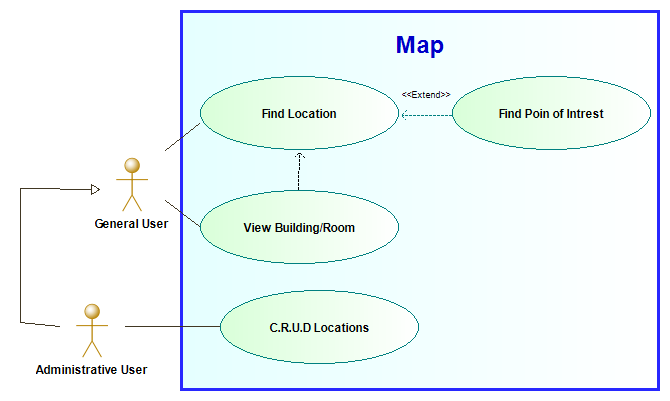
\includegraphics[width=\textwidth]{images/Map_Use_Case_Diagram.png}
\begin{center}
	Figure 8: Map Module Use Case
\end{center}

	{The map system will contain all the stationary information regarding the system, thus it contains the digital information that maps to the real world. A use case exists wherein the general user will be able to search for locations on campus. This use case will be extended to provide functionality whereby the general user can search for specific points of interest on campus, such as toilets and coffee shops. The map system will also allow general users to view buildings and rooms as well as their related information such as historical facts. The map system will also provide the administrative user the rights to C.R.U.D. locations and information regarding those locations.
}